\documentclass[12pt]{article}
%\usepackage[margin=0.8in]{geometry}
\usepackage{amsmath,amssymb}
\usepackage{graphicx}
\usepackage{float}
\usepackage{xcolor}
\usepackage[margin=2cm]{geometry}
\geometry{margin=1in, headsep=0.25in}
\usepackage{titlesec}
\titlespacing*{\section}{0pt}{3.5ex plus 1ex minus .2ex}{3ex plus .2ex}
\newcommand{\xpo}{x_{\mathbb{P}}}

\title{Diffractive charm: status}
\author{}
\date{\today}

\begin{document}
%\maketitle

\textit{ Paul: How much is the result sensitive to the precise value of this cut-off? 
Since the GDTMD is steeply falling at large $K_\perp$ I would expect that this upper
 limit does not really matter (as long as $p\gg Q_s$) and we could in fact always in
 tegrate up to infinity. Would be interesting to check. Also, is the 
 condition $p\gg Q_s$ always satisfied in the predictions and comparisons to data?}

\section*{1. $p\gg Q_s$ ?}

We define $Q_s^2=2/r_s^2$, where $N(r_s,\xpo)=1-e^{-1/2}$, for the quark dipole $N$ (quark DTMD) and
the gluon dipole $N_A=2N-N^2$ (gluon DTMD). $N_A$ gives a larger $Q_s$.

$Q_s$ grows as $\xpo$ decreases, and the smallest $\xpo$ at each $p_\perp$ is $\xpo^{\min}=M_{c\bar c}^2/W^2$.
In the figure we show $Q_s(\xpo^{\min})$, the largest $Q_s$, for $y=0$ (lower edge) to $y=3$ (upper edge).

\begin{figure}[h]
\centering
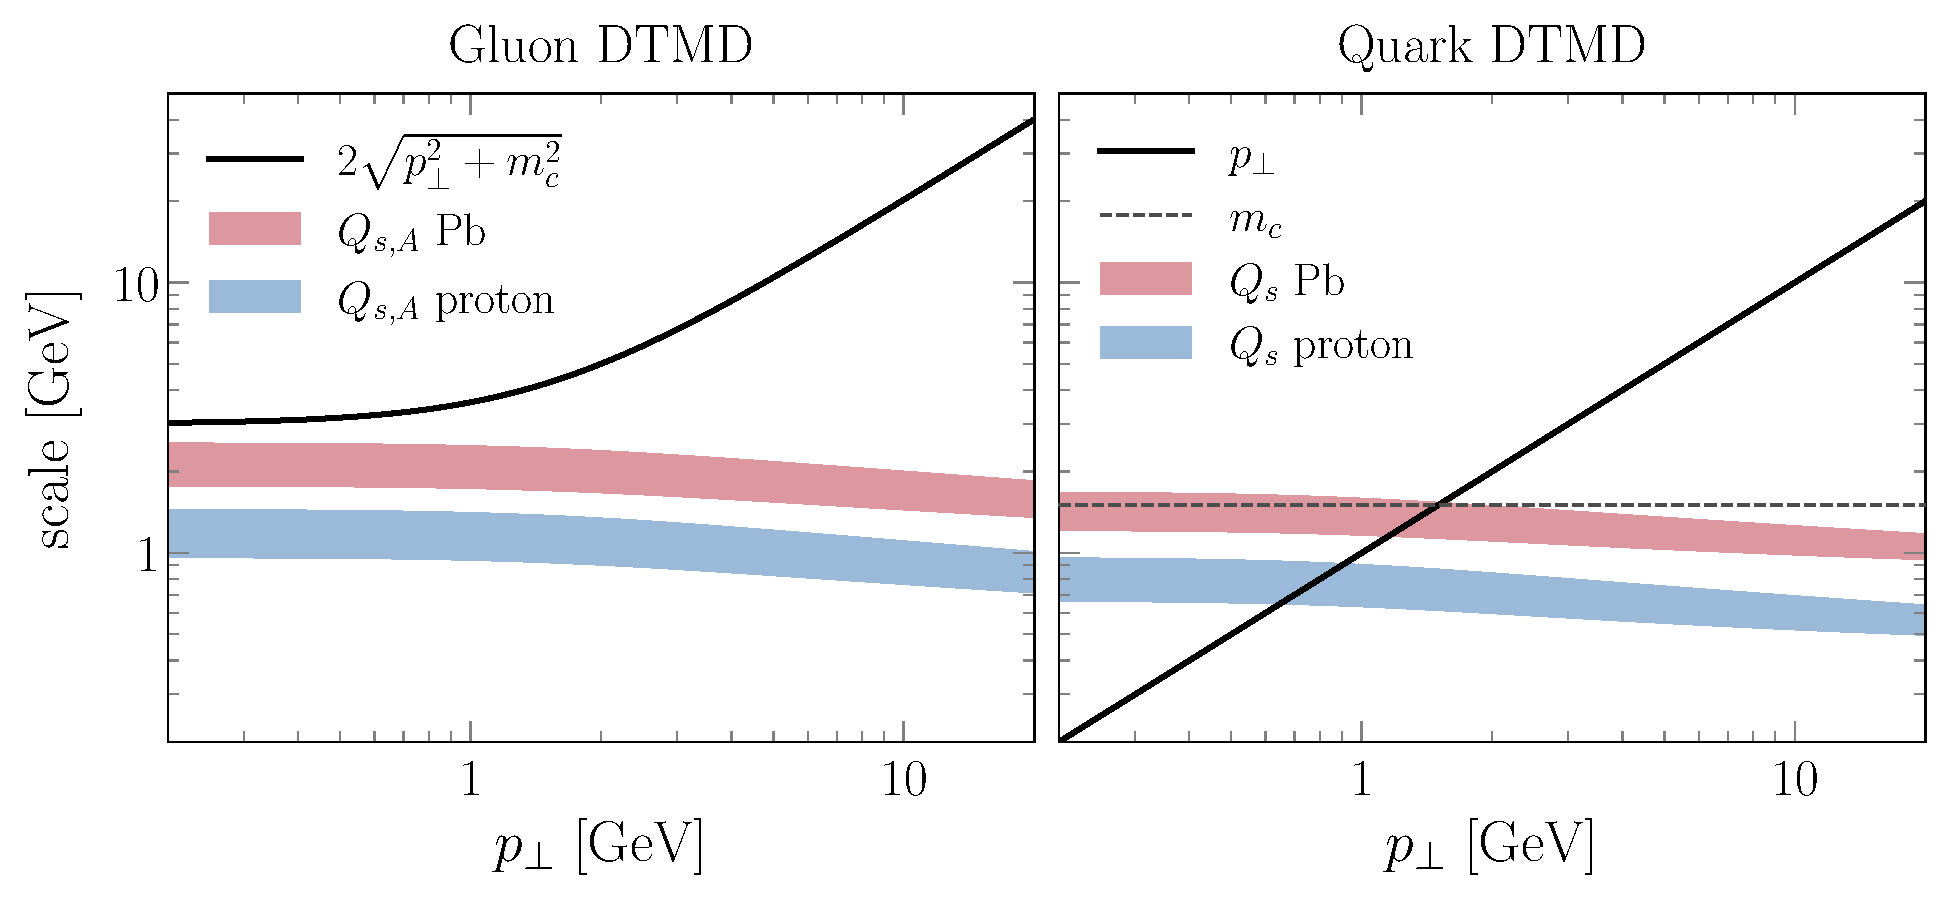
\includegraphics[width=0.95\textwidth]{../plots/correlation_limit.pdf}
%\caption{%Hard scale of the gluon DTMD ($2m_T$, left) and of the quark DTMD ($p_\perp$, right) compared with
%the saturation scale of the proton and of Pb.}
%\caption{Hard scale (black) of the gluon DTMD (left) and of the quark DTMD (right) compared with $Q_s$ of the
%proton (blue) and of Pb at $b=0$ (red). The bands span $y=0$ (lower edge) to $y=3$ (upper edge), with $Q_s$ at
%the smallest $\xpo$ reached at each $p_\perp$.}
\end{figure}

\begin{itemize}

\item Correction in the GDTMD: the hard scale is $M_{c\bar c}^2=m_T^2/(z\bar z)$ with
  $m_T^2=p_\perp^2+m_c^2$, that is,  $M_{c\bar c}=2m_T$ at $z=0.5$.
\item In the D$^0$ spectra, we could add 

$\rightarrow$ GDTMD for $p_\perp \geq3$~GeV, where the dependence on the $K$-cut is below 10\%.
  
 $\rightarrow$  QDTMD  for $p_\perp\geq5$~GeV, where the dependence on the $K$-cut is
  10--20\%.

 $\rightarrow$  Exclusive for $p_\perp < 3$~GeV.

\end{itemize}

\section*{2. Quark DTMD contribution}

\begin{figure}[h]
\centering
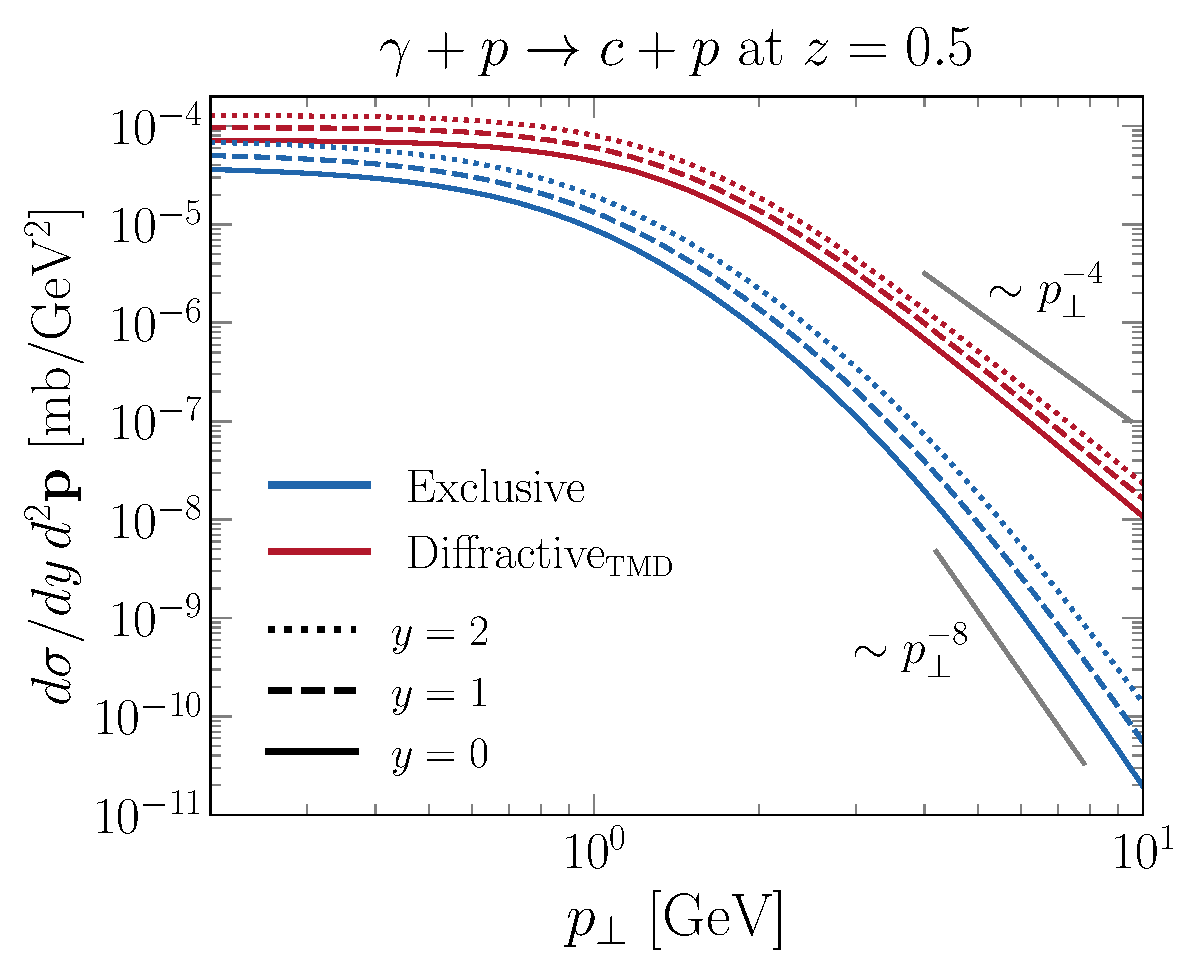
\includegraphics[width=0.55\textwidth]{../plots/charm_fixed_qp.pdf}
%\caption{Charm cross section on a proton at fixed $q^+=2p^+$ ($z=\tfrac12$), no photon flux and no
%fragmentation.}
\end{figure}

\begin{itemize}
%\item The diffractive ($c\bar c g$) channel is larger than the exclusive ($c\bar c$) one at all $p_\perp$:
%  by a factor $\approx2$ at low $p_\perp$ and by more than an order of magnitude above 2~GeV.
\item Before, the gluon DTMD contribution was smaller than the exclusive at low $p_\perp$ because I was missing 
 part of the integral by setting the upper limit at $K_\perp\leq p_\perp$ (even though we do not apply diffractive $q\bar{q}g$ at low $p_\perp$). From
  $p_\perp\approx3$~GeV the dependence on the cut is below 10\%.
%\item Exclusive falls as $p_\perp^{-8}$, diffractive as $p_\perp^{-4}$.
\item The quark DTMD ($p_\perp\geq5$~GeV) has the same momentum dependence at large $p_\perp$, but is less than $1\%$ of the diffractive cross section
  ($\approx2\%$ for Pb).
  
  This could be because of the $x=M^2/(\xpo W^2)\propto1/\xpo$ dependence of the TMDs:
  \begin{itemize}
  \item In our previous paper (Sec.~4.3) we show that the quark DTMD is proportional to $x$ at small $x$,
    in contrast with the GDTMD. Since $x\propto1/\xpo$, the quark DTMD only
    contributes near the smallest $\xpo$ allowed at each $p_\perp$ ($\xpo^{\min}=M_{c\bar c}^2/W^2$, where $x\sim1$),
    whereas the gluon DTMD contributes over the whole $\xpo$ range.
  \item Less relevant are the charm mass, which suppresses the quark DTMD (by $\sim(Q_s/m)^4$ for $m\gg Q_s$,
    Eqs.~(4.59)--(4.60) in our previous paper), and the adjoint dipole $N_A\approx2N$ in the gluon DTMD.
  \end{itemize}
\end{itemize}

\begin{figure}[H]
\centering
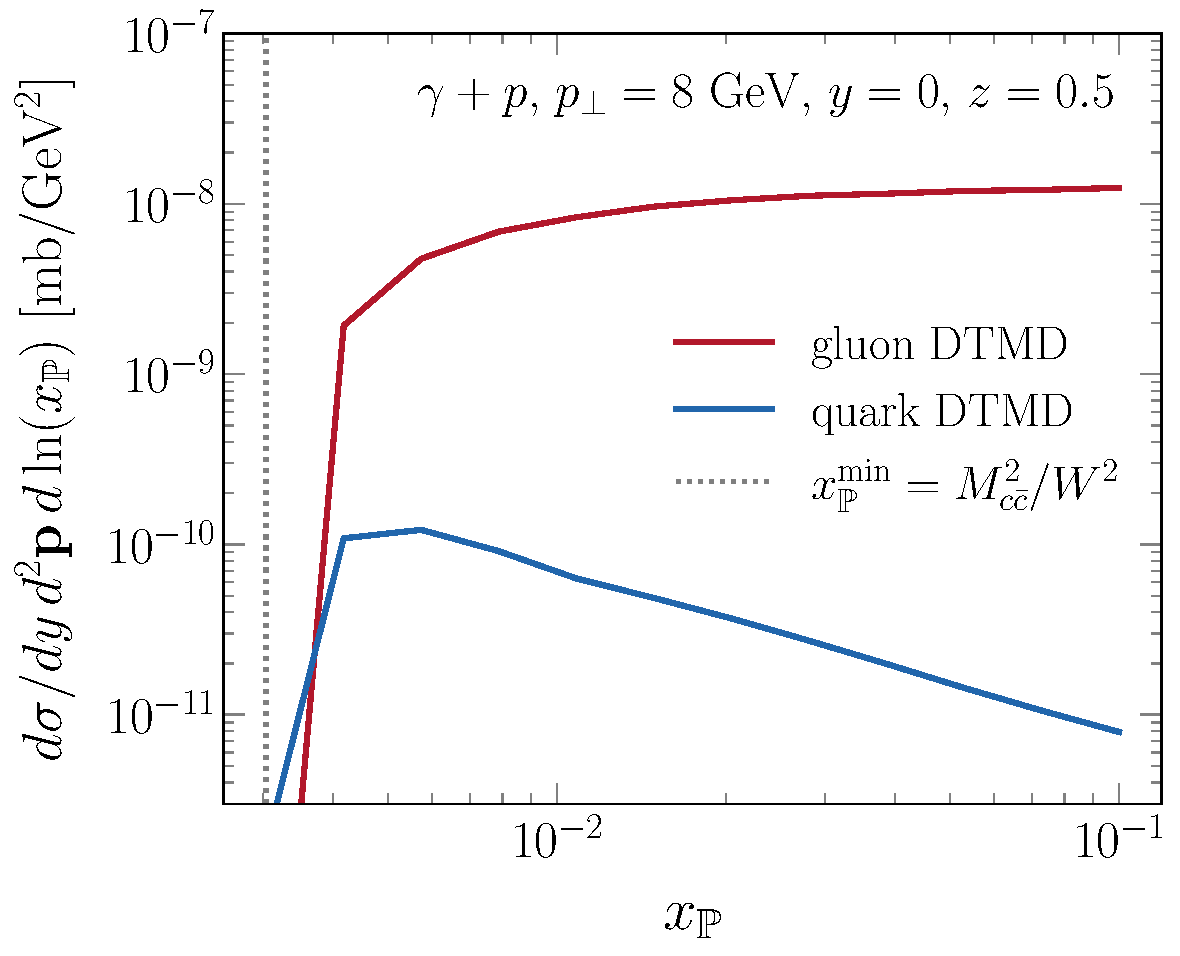
\includegraphics[width=0.5\textwidth]{../plots/xpom_quark_vs_gluon.pdf}
\end{figure}


\section*{3. Large-$p_\perp$ tail of the exclusive cross section}

\begin{figure}[H]
\centering
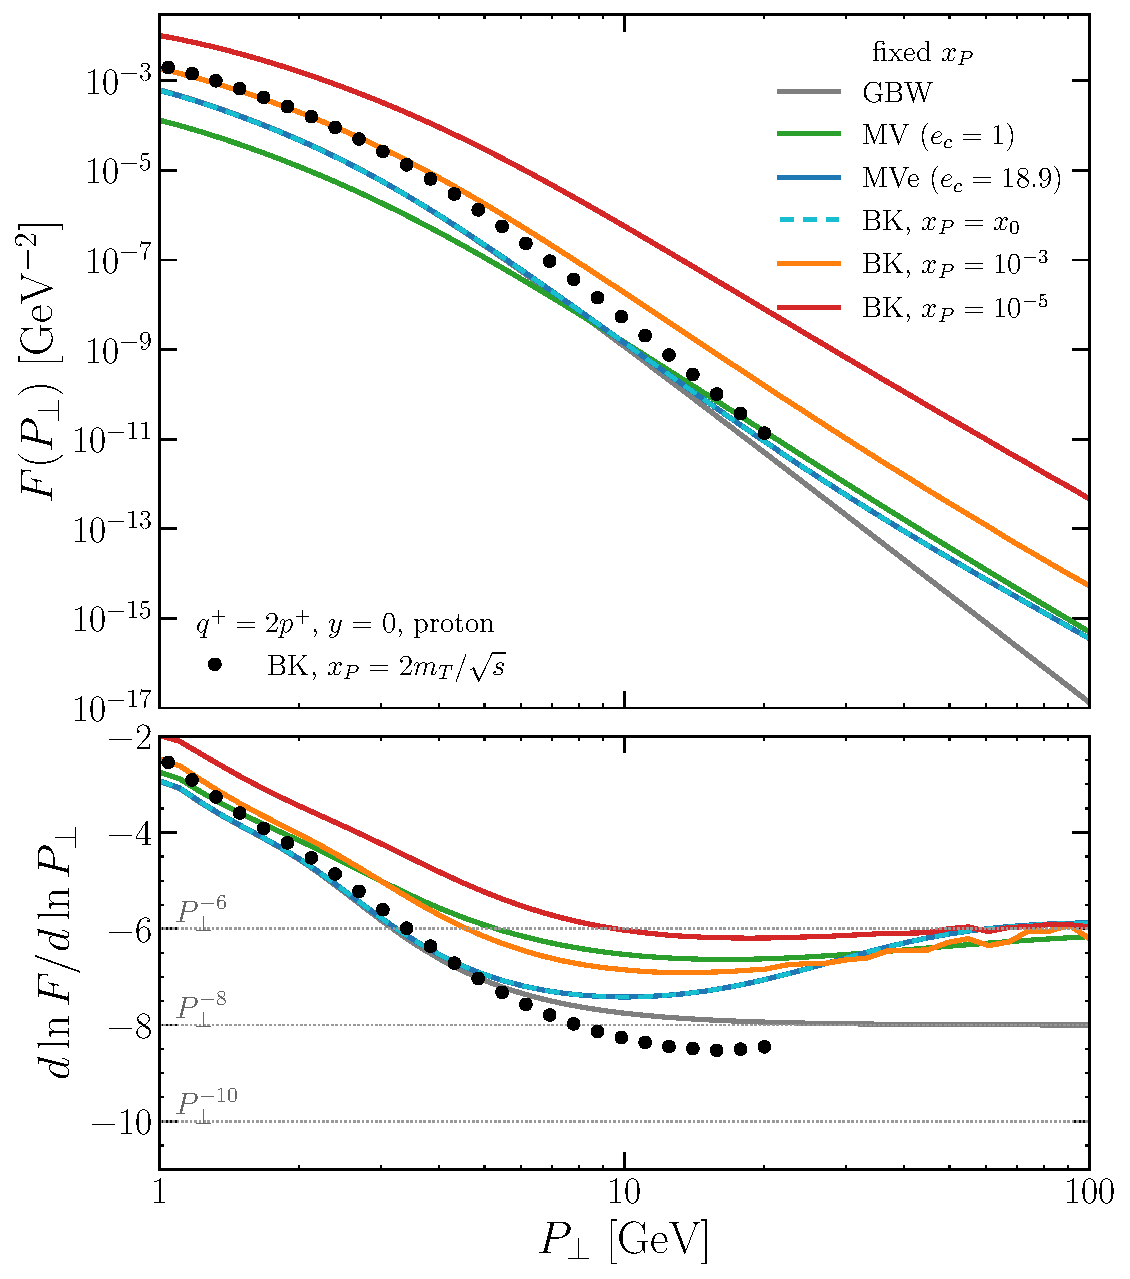
\includegraphics[width=0.75\textwidth]{../plots/exclusive_tail.pdf}
%\caption{Exclusive $c\bar c$ cross section on a proton (top) and its local power (bottom) for several dipole
%amplitudes. Dots: our code, where $\xpo=2m_T/\sqrt s$ grows with $p_\perp$.}
\end{figure}

Agreement with Paul's calculation:
\begin{itemize}
\item GBW: the tail goes like $p_\perp^{-8}$  ($m^2Q_s^4/p_\perp^8$).
\item Massless GBW (I take $\bar Q=m_c$ to compare): it goes like $p_\perp^{-10}$.
\item MVe: the log in $N(r)$ acts like $\gamma\neq1$, so the $Q_1$ term gives a $p_\perp^{-6}$ tail. But it
  is only greater above $\approx30$~GeV. Below, the mass dependent $Q_0$ term dominates.
\item BK makes the tail a bit flatter.
\item Dots (our code): $\xpo$ grows with $p_\perp$, so there is less evolution at large $p_\perp$ and the
  prediction goes like $\approx p_\perp^{-8.5}$.
\end{itemize}

\end{document}
